%-------------------------------------------------------------------------------
\section{Evaluation}
\label{s:eval}
%-------------------------------------------------------------------------------

This section answers the following questions:
\begin{enumerate}
    \item Does \schedbe{} honor LC's CPU reservations in presence of BE?
    \item Can parked processes resume correctly? How many resources does it used
    while parked?
    \item How much does \schedbe{} cost?
    \item How does \schedbe{}'s ability to limit the impact BE has on LC compare
    to that of \schedidle{}?
\end{enumerate}

All the graphs in this paper run on Linux version 6.14.2, the baseline version
that our implementation builds on. We run the experiments on two machines with
Intel(R) Xeon(R) CPU E5-2680 v4, running at 2.40GHz, with 2 NUMA nodes with 14
cores each, and 2 hyperthreads per core. Unless otherwise specified, most
experiments run on four cores on the same NUMA node. The two machines are
connected by a 100Gbps network connection, and the ping time between them is
0.2ms. The graphs are generated from one run of the experiment.

\subsection{Does \schedbe{} isolate?}

\begin{figure}[t]
    \centering
    \begin{subfigure}{\columnwidth}
        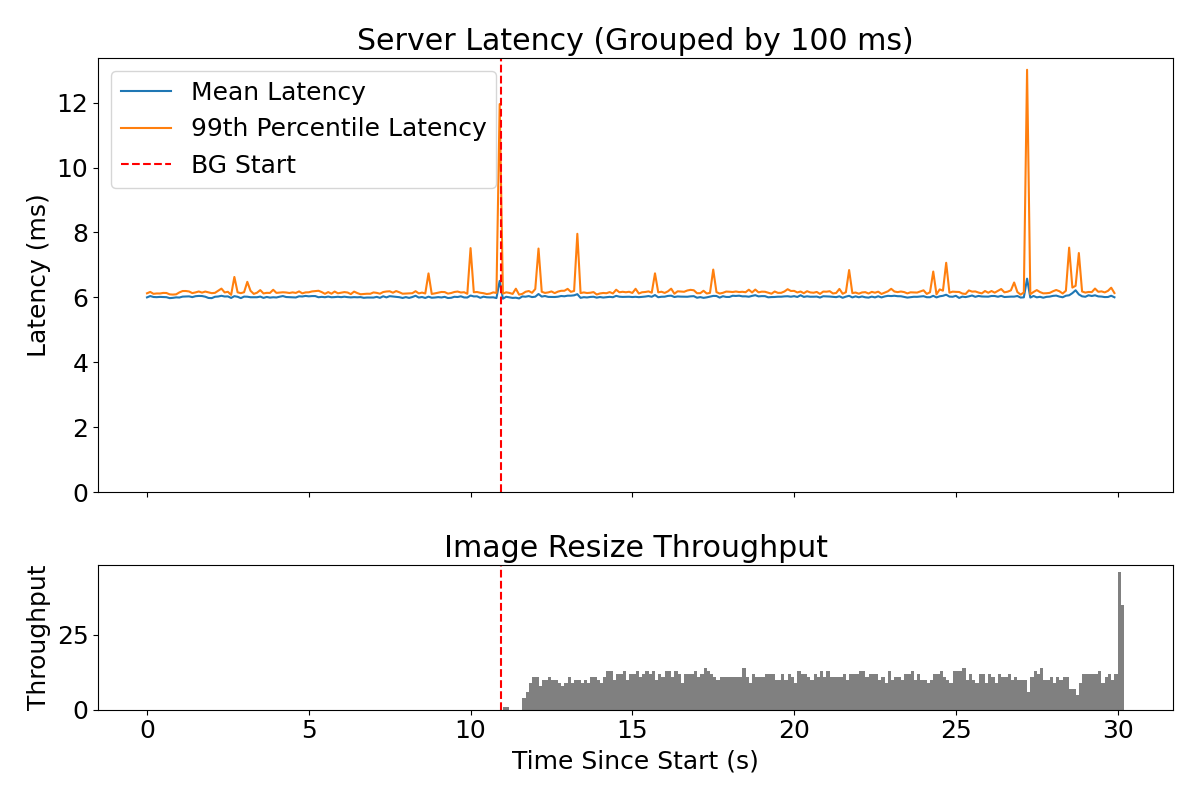
\includegraphics[width=\columnwidth]{graphs/srv-bg-schedbe-low.png}
        \caption{Low load (85\%)}\label{fig:srv-bg-schedbe-low}
        \vspace{12pt}
    \end{subfigure}
    \begin{subfigure}{\columnwidth}
        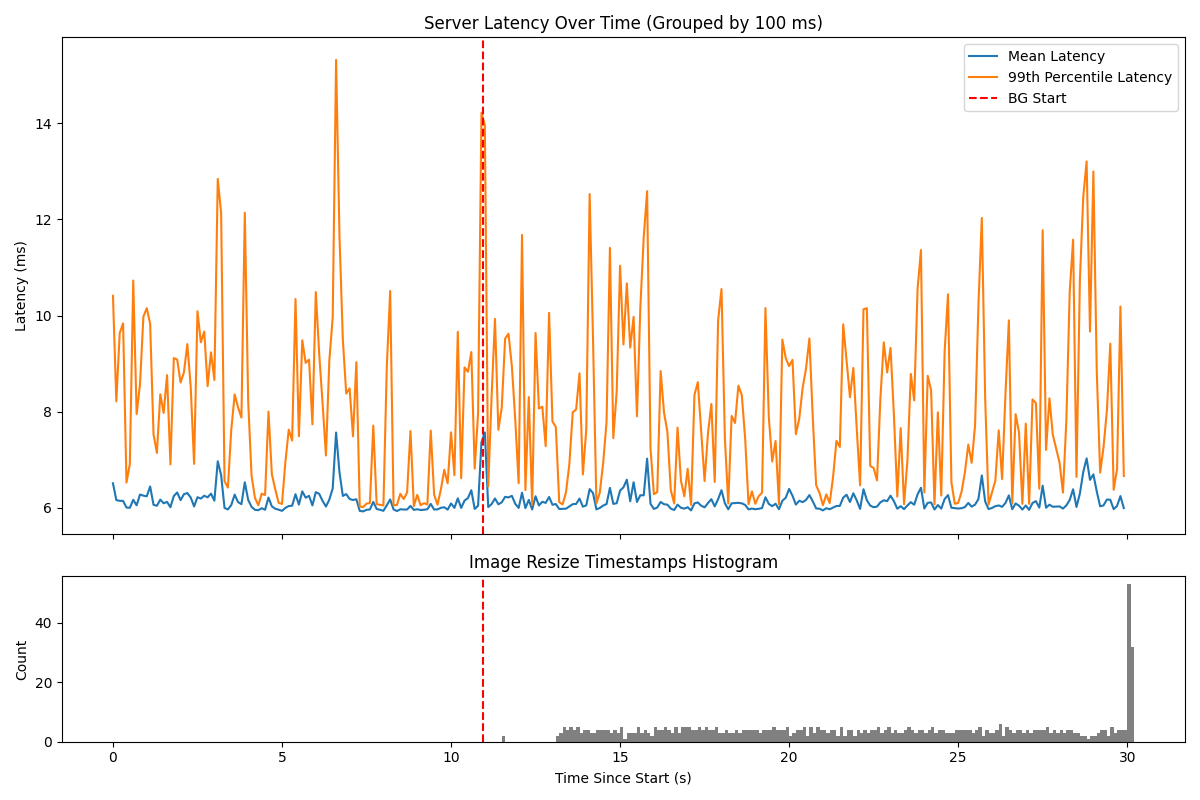
\includegraphics[width=\columnwidth]{graphs/srv-bg-schedbe-high.png}
        \caption{High load (95\%)}\label{fig:srv-bg-schedbe-high}
    \end{subfigure}
    \vspace{4pt}
    \caption{ \schedbe{} does a good job of isolating the server's latencies
     from the load from best effort jobs}\label{fig:srv-bg-schedbe}
\end{figure}

\begin{figure}[t]
    \centering
    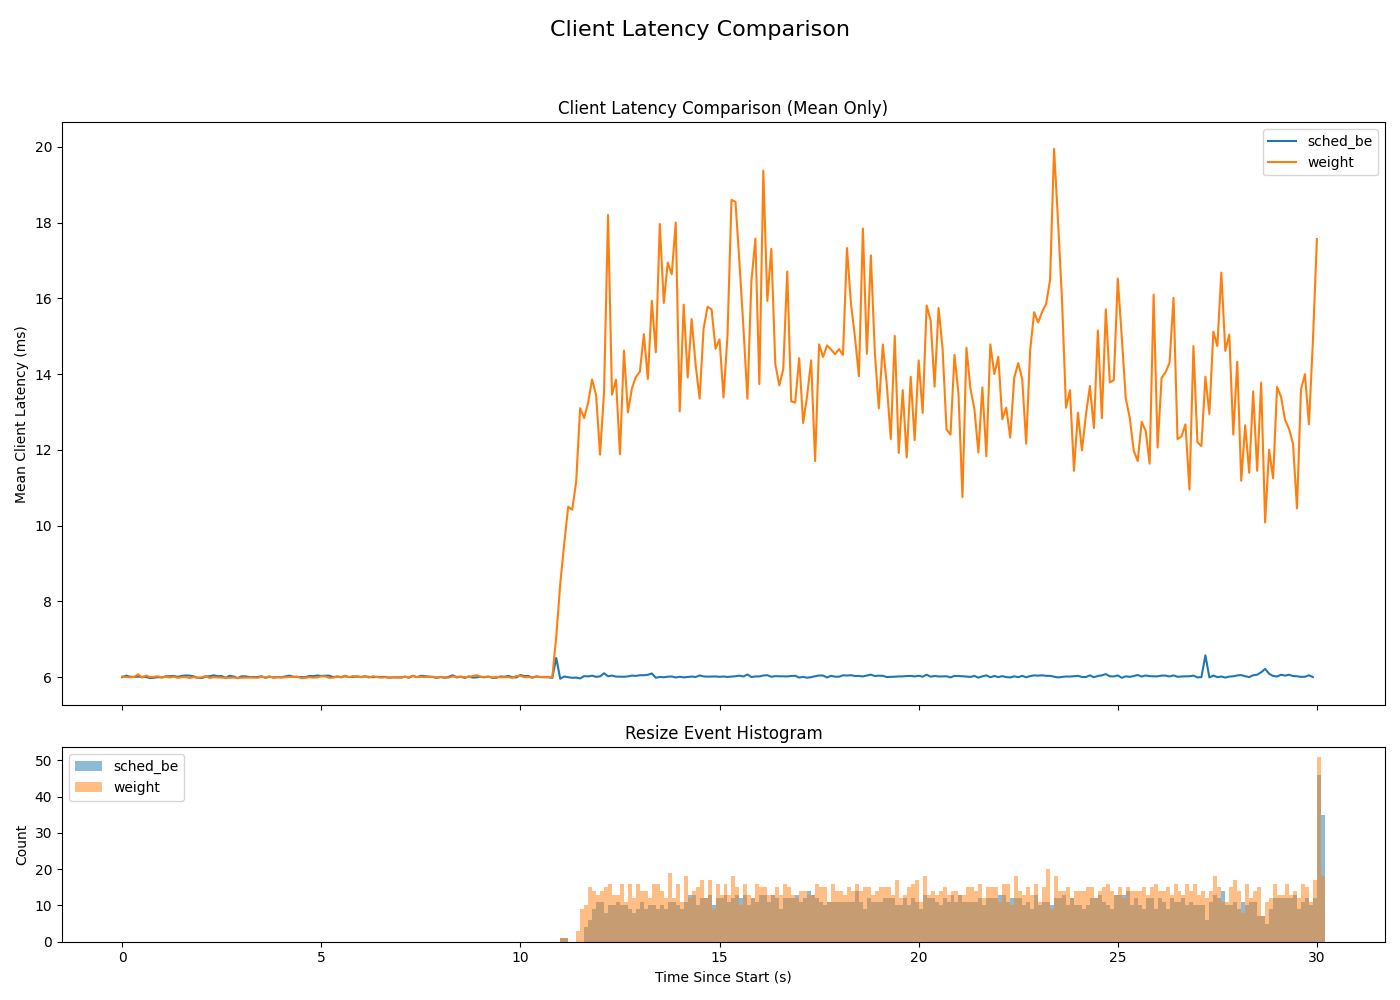
\includegraphics[width=\columnwidth]{graphs/srv-bg-cmp-unedited-schedbe.png}
    \caption{A direct comparison between the server latencies when using the
    existing \cgroups{} weights versus \schedbe{} }\label{fig:srv-bg-cmp-unedited-schedbe}
\end{figure}

\begin{figure}[t]
    \centering
    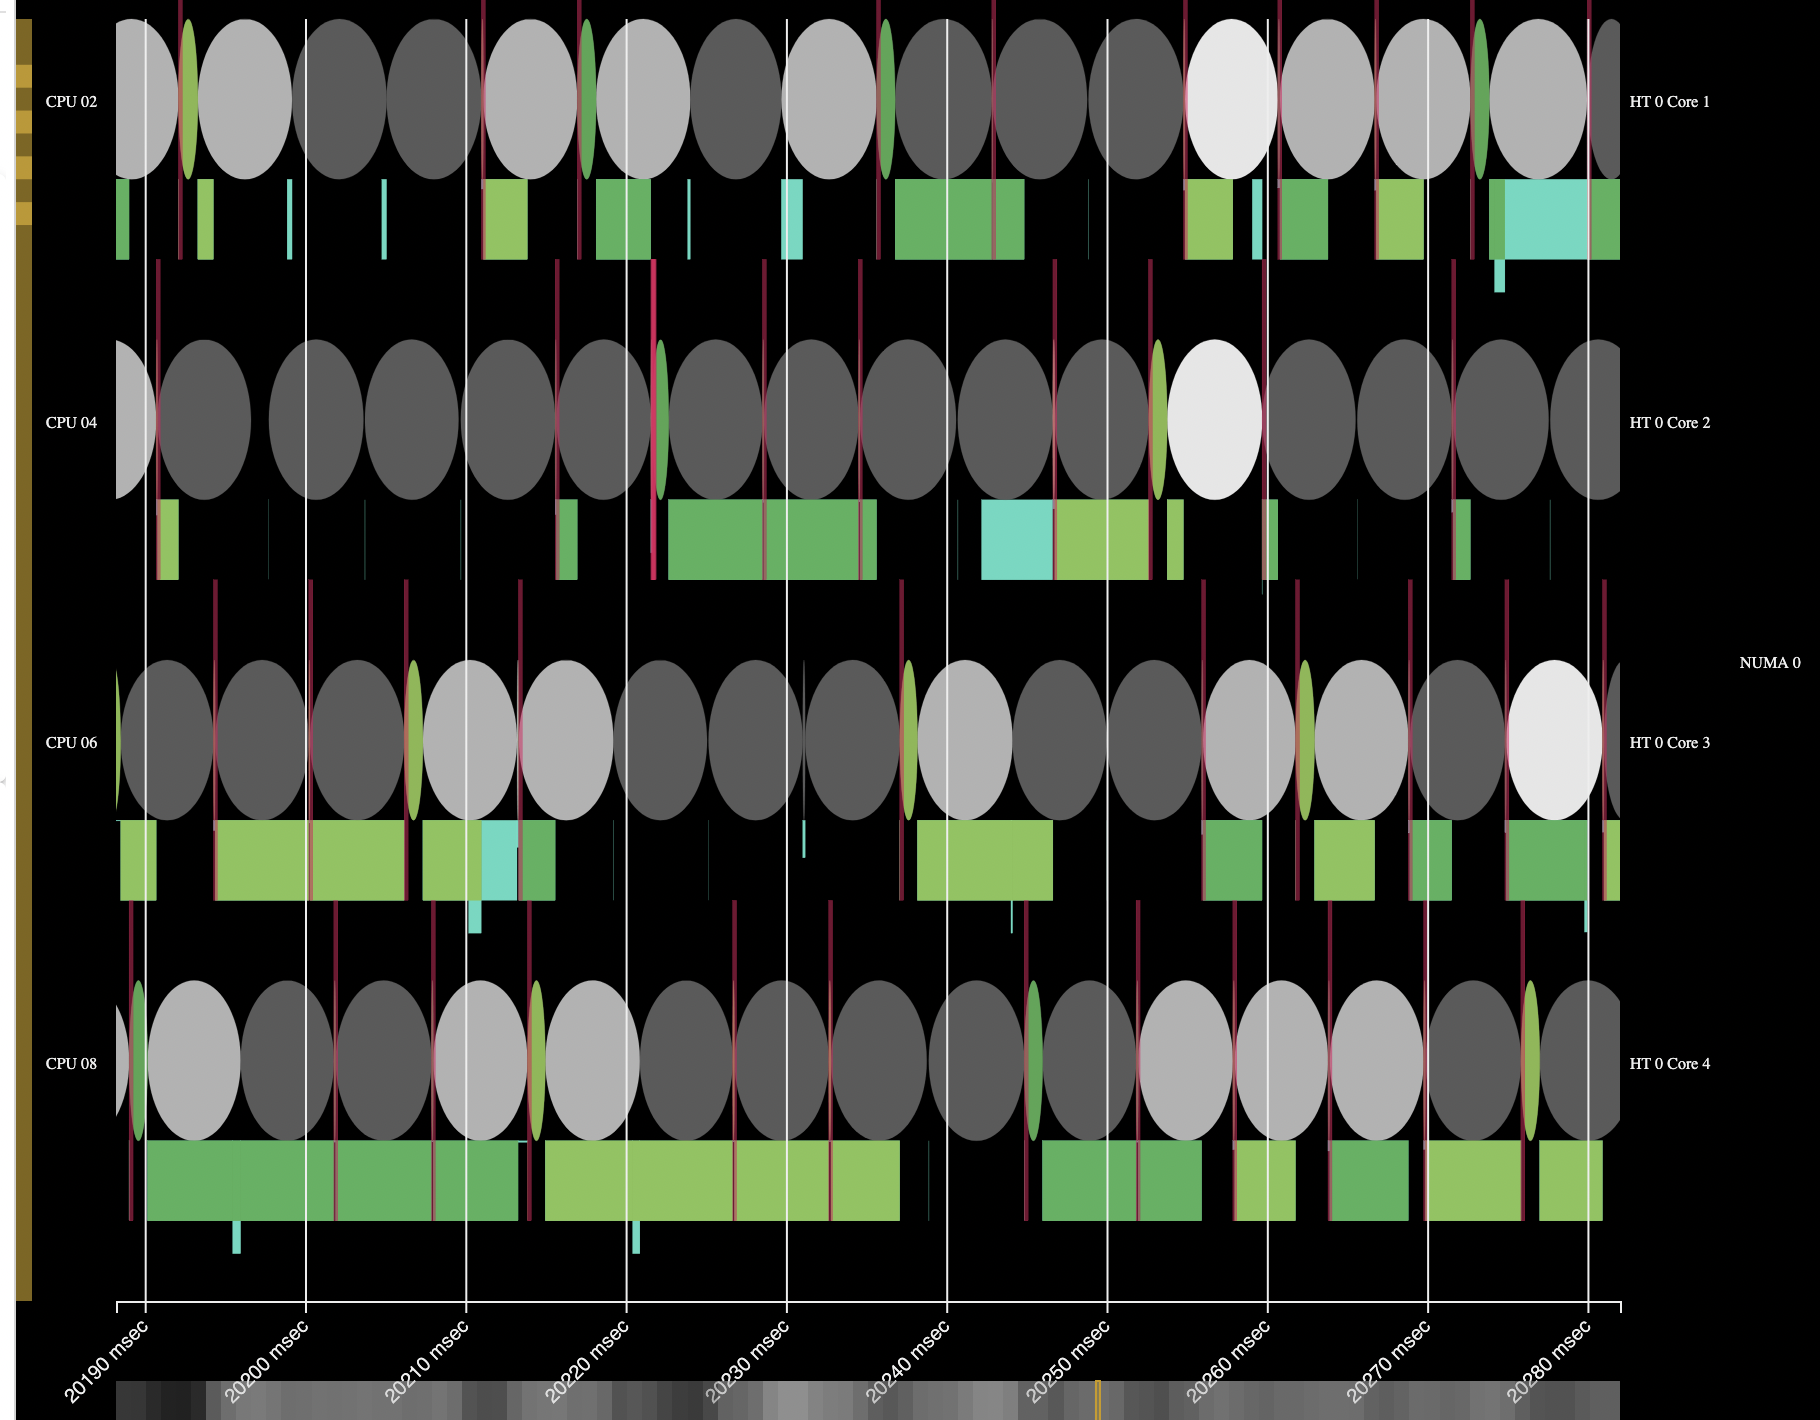
\includegraphics[width=\columnwidth]{graphs/schedviz-schedbe.png}
    \caption{BE threads only run in the gaps when there are no queued LC threads
    on any core }\label{fig:schedviz-schedbe}
\end{figure}

We run the microbenchmark experiment from \autoref{fig:srv-bg-weight-150} using
\schedbe{}. We can see the resulting performance in
\autoref{fig:srv-bg-schedbe}, and \autoref{fig:srv-bg-cmp-unedited-schedbe}
shows a direct comparison between the original benchmark run on \cgroups{}
weights and running it using \schedbe{}. As desired, the latency of the server
remains stable after the background tasks start. 

The background task still runs: the lower part of each graph still shows
iterations of image resizing being done. The difference is that now the
background tasks will reliably get interrupted when the LC server has a request
to process. \autoref{fig:schedviz-schedbe} shows the interruption happening in
an outtake of a schedviz visualization. The green BE processes run only in the
gaps where there is no queued LC process, and are immediately preempted when one
wakes up, on whatever core that may be. The vertical red lines show when the
\exit{} path \schedbe{} introduced runs (\ie{} when the core has chosen intially
to run a BE process after having previously run LC). As we can see, this line is
sometimes followed by running the BE, but often by the core running an LC
process, meaning that it succesfully found and stole a queued and waiting LC
thread.

\begin{figure}[t]
    \centering
    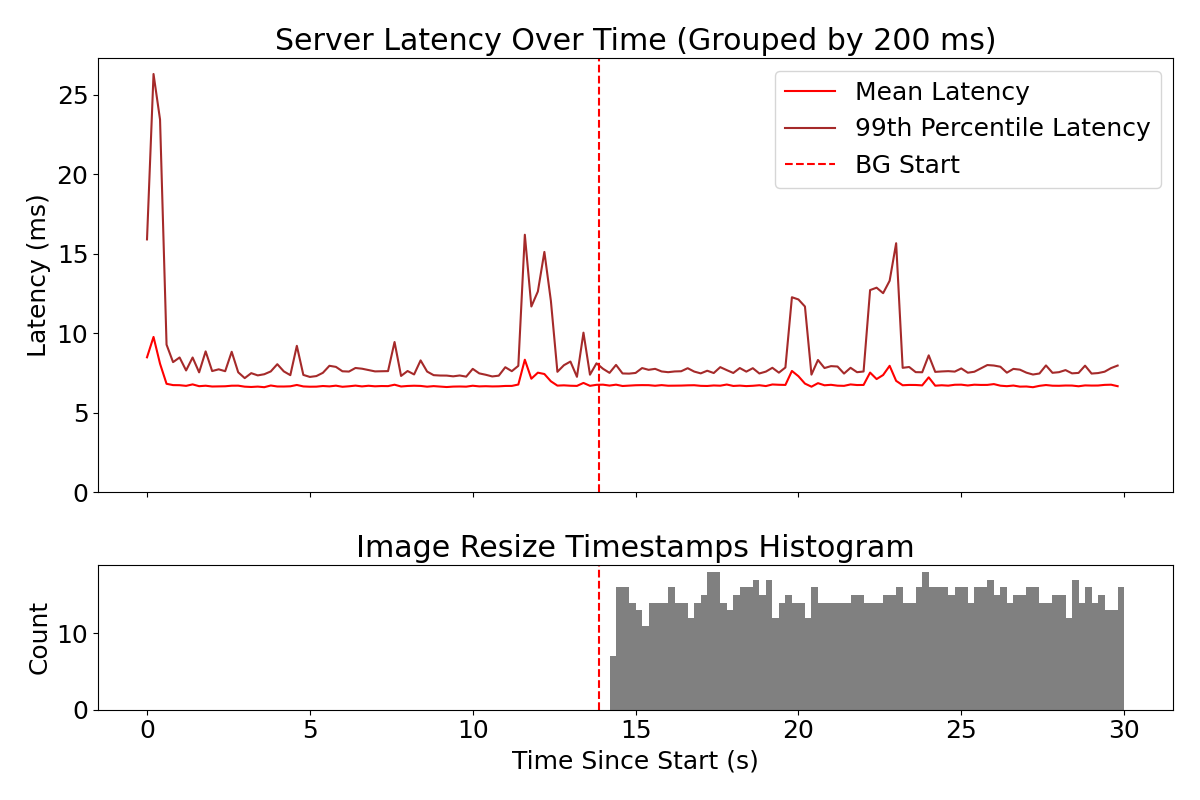
\includegraphics[width=\columnwidth]{graphs/kubernetes-schedbe.png}
    \caption{The same experiment as in \autoref{fig:kubernetes-unedited}, but
    running the BE as a \schedbe{} task}\label{fig:kubernetes-schedbe}
\end{figure}

We also run the Kubernetes application from \autoref{fig:kubernetes-unedited}
using \schedbe{}. The results are in \autoref{fig:kubernetes-schedbe}. We can
see that again the latency profile of the LC web application looks largely the
same before and after starting the image resize job.\hmng{run for longer and/or
get concrete numbers for how much it increases, vague hedging (largely, not
entirely) is not good} It is not entirely without spikes, but the spikes come
from interference with Python runtimes and Kubernetes controllers, and are the
same before and after starting the BE tasks. Importantly, the baseline median
latency of the LC web application stays stable at around 7.4ms after starting
the the BE image resizing. 

\subsection{Can parked processes resume correctly? How much do they cost while
parked?}\label{ss:eval:parking}


\begin{figure}[t]
    \centering
    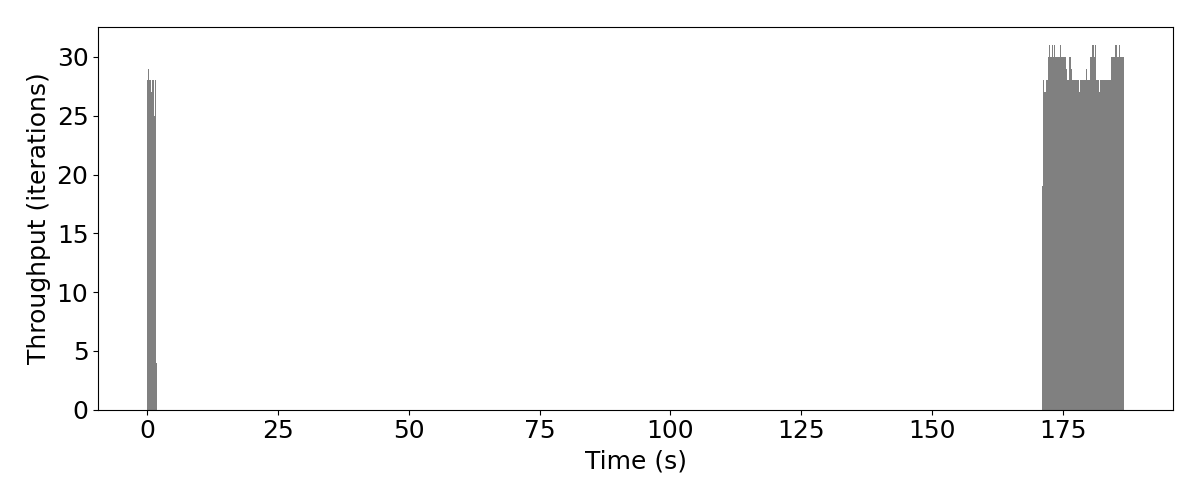
\includegraphics[width=\columnwidth]{graphs/parked-kubernetes.png}
    \caption{A \beclass{} process in a Kubernetes pod, parked while the
    antagonist runs and then resuming}\label{fig:parked-kubernetes}
\end{figure}

We investigate parking by running a BE Kubernetes pod alongside an antagonist,
and find that even after being parked for multiple minutes in the middle of
processing a request, the BE job is able to resume and return the final result
to the client. 

\autoref{fig:parked-kubernetes} shows the throughput over time of an image
resize job running in a BE container running as \schedbe{}. A couple seconds
after sending a request to the image resize pod, we start an entirely CPU-bound
antagonist on the same set of cores as the BE is running. We can see that the
image resize job is completely paused for about two and a half minutes, until
the antagonist is done running. The job then continues and completes. The client
connection did not experience any issues, even when setting the TCP keepalive
timeout to expire within duration the BE spent being parked.

\begin{figure}[t]
    \centering
    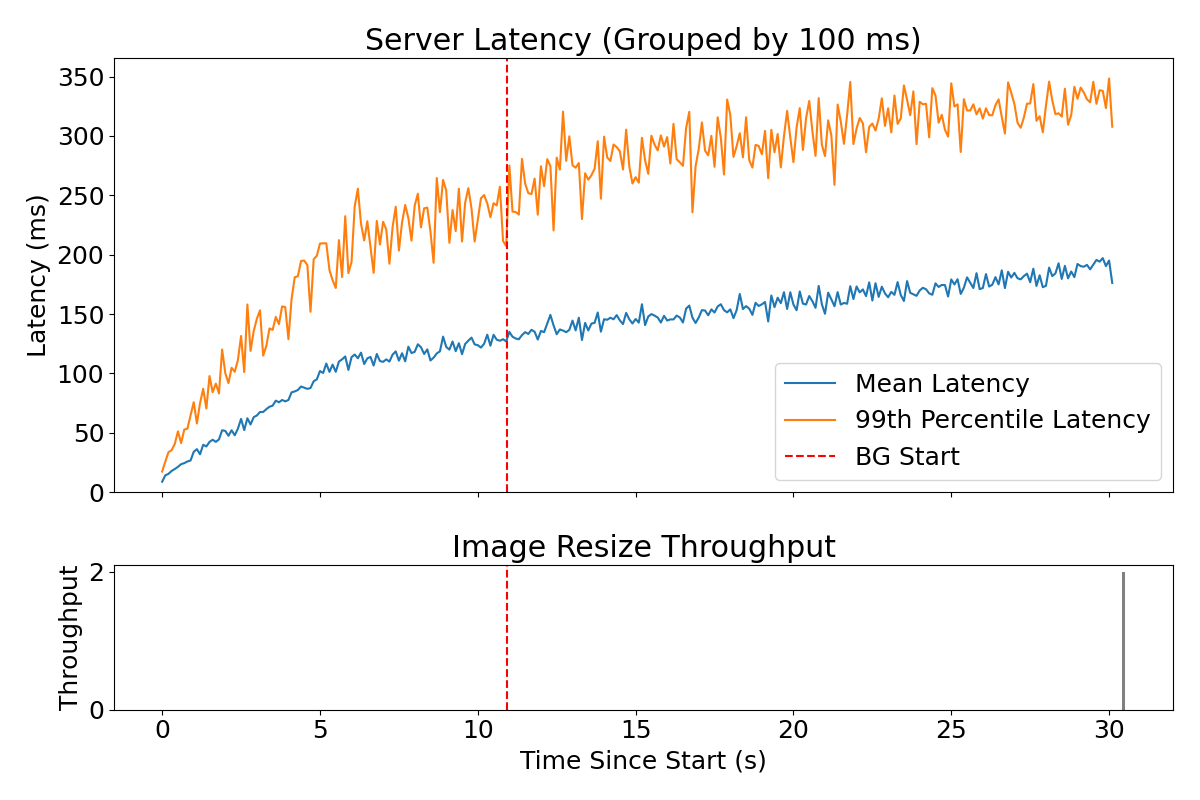
\includegraphics[width=\columnwidth]{graphs/overload-schedbe.png}
    \caption{BE in \schedbe{}, no throttling}\label{fig:overload-schedbe}
\end{figure}

\autoref{fig:overload-schedbe} shows how parking enables the latency critical
server to keep its reservation even under sustained extremely high load. We run
the same experiment as \autoref{fig:overload-rt}, but now instead instead of
throttling the server, \schedbe{} parks the best effort processes. Notice that
the \schedbe{} image resize job does not make progress until the very end, when
the server is done processing the requests. The difference is stark: in both
experiments, the open-loop client sent the same amount of requests with the same
amount of time in between them, but when the LC was throttled it took the server
35s to process all the requests, with a final latency of >1s, and with parking
the server finished the client load in 31s with a final avg latency of <200ms. 



\subsection{Cost breakdown of \schedbe{}}

The cost of \schedbe{} is can be broken down into the three checks that make up
the priority enforcement:

\begin{enumerate}
    \item \local{} adds a small amount of compute overhead on each scheduling
    decision to determine threads' priorities. This is a small amount of code we
    do not expect to impact latency
    \item \entry{} adds no new latency to Linux, which already implements
    \entry{} for \schedidle{}
    \item \exit{} adds overheads in two places: one is the cross-core check that
    each happens at each class boundary crossing, and the other is the overhead
    of the migration should it decide to steal a \schednormal{} process
\end{enumerate}

We look at how often the \exit{} check happens as well as how often it chooses
to steal in the Kubernetes experiment. The overhead of stealing the LC job is
known, and is a complicated function of the CPU architecture and which cores it
is moving between (\eg{} how much memory hierarchy do the two cores share).

% Please add the following required packages to your document preamble:
% \usepackage[normalem]{ulem}
% \useunder{\uline}{\ul}{}
\begin{table}[t]
    \centering
    \begin{tabular}{|l|l|l|}
        \hline
                & \# times runs & \# times successful \\ \hline
        \entry{} & $\sim$60K    & $\sim$12.5K         \\ \hline
        \exit{}  & $\sim$20K    & $\sim$10K          \\ \hline
    \end{tabular}
    \vspace{10pt}
    \caption{The \exit{} and \entry{} checks are effective, significant
    fractions of the times they run lead to stealing a queued LC
    thread/interrupting a currently running BE one}\label{tab:check-counts}
\end{table}

In the span of the 30 seconds the Kubernetes experiment takes to run, and across
the four cores it runs, we see the following: scheduling happens around 110K
times, which is a little less than once per ms on each core. The \entry{} check
happens $\sim$60K times, or about twice a ms. This makes sense: the client sends
a request every 2ms which will cause a server thread wakeup, and the software
stack includes Linux, Docker, and Kubernetes, all of which have worker threads.
Of those 60K \entry{} checks, 12.5K find an idle runqueue. The \exit{} check
happens fewer times, around 20K times, of which approximately half lead to
stealing a \schednormal{} task.

We can see that the \entry{} and \exit{} checks happen less than scheduling does
by more than half. This result demonstrates that enforcing prioritization
between LC and BE via priority classes requires much fewer global cross-core
runqueue checks than doing so at every scheduling decision.

The other takeaway is that, under high load, the \exit{} check is effective:
around half of the time, the scheduler found a queued LC thread on another core.
Without the check, each of those would have led to a priority inversion.


\subsection{Comparison with \schedidle}\label{ss:eval:schedidle}

As discussed in \autoref{s:implementation}, \schedidle{} implements the \entry{}
check, but not the \exit{} check or strict local priorities.

\begin{figure}[t]
    \centering
    \begin{subfigure}[t]{\columnwidth}
        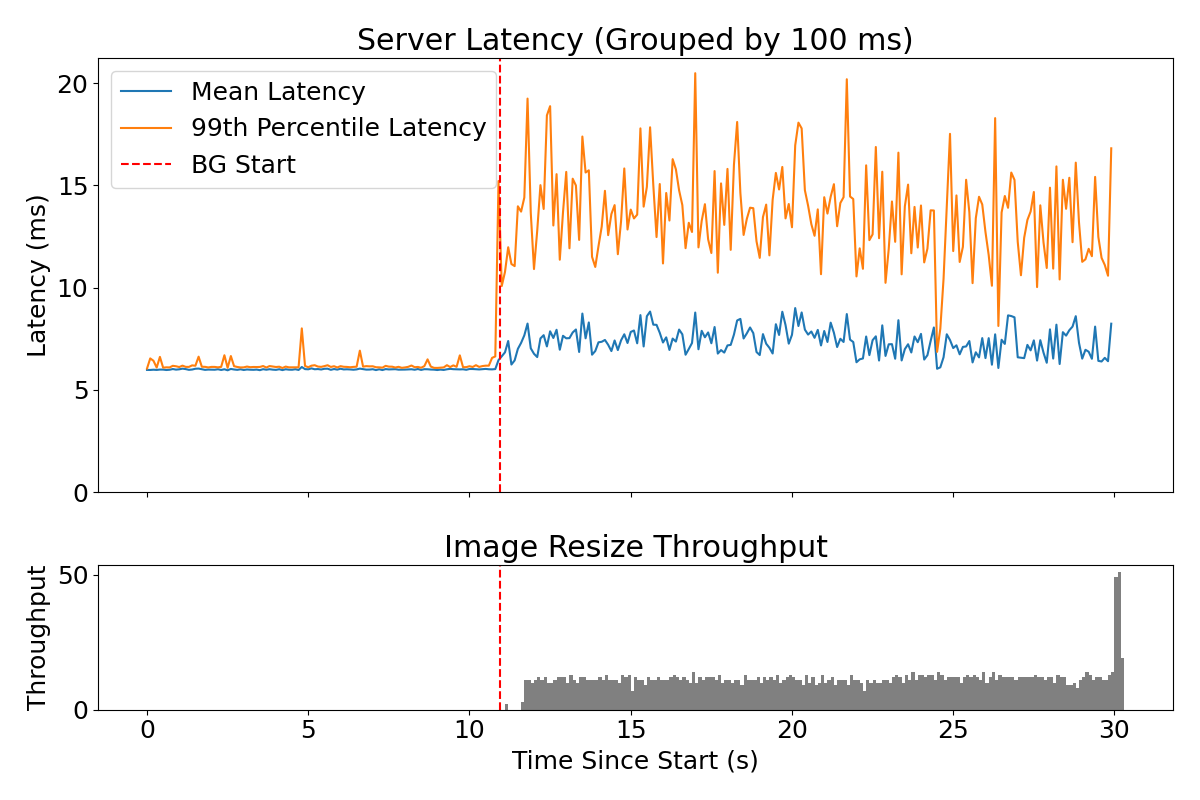
\includegraphics[width=\columnwidth]{graphs/srv-bg-idle-low.png}
        \caption{\schedidle{} in low load (85\%)}\label{fig:srv-bg-idle-low}
        \vspace{12pt}
    \end{subfigure}
    \hspace{\fill}
    \begin{subfigure}[t]{\columnwidth}
        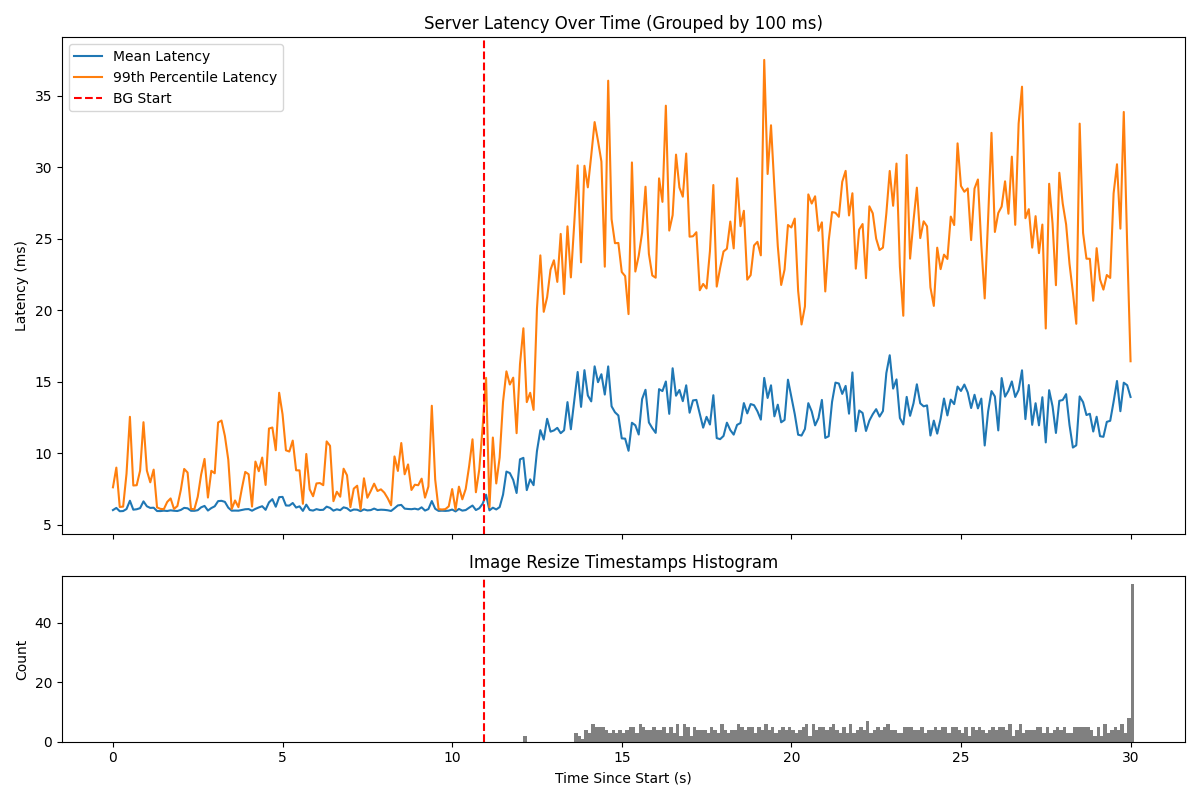
\includegraphics[width=\columnwidth]{graphs/srv-bg-idle-high.png}
        \caption{\schedidle{} in high load (95\%)}\label{fig:srv-bg-idle-high}
        \vspace{12pt}
    \end{subfigure}
    \hspace{\fill}
    \begin{subfigure}[t]{\columnwidth}
        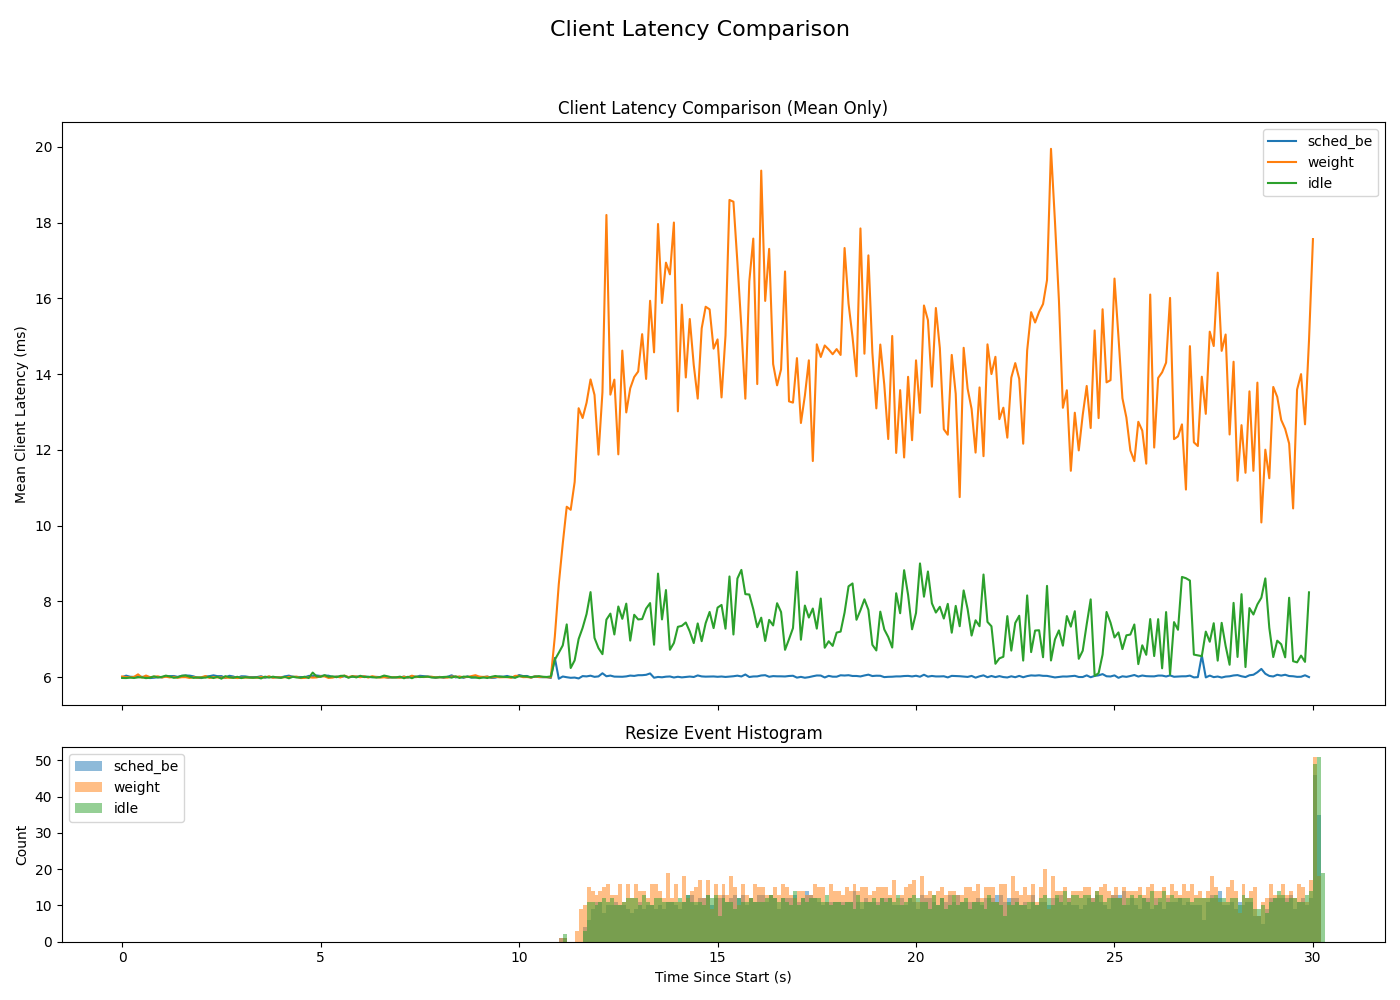
\includegraphics[width=\columnwidth]{graphs/srv-bg-cmp-all.png}
        \caption{Comparison of mean latency of the low load setting for weights,
        \schedidle{}, and \schedbe{}}\label{fig:srv-bg-cmp}
    \end{subfigure}
    \vspace{4pt}
    \caption{}\label{fig:srv-bg-idle}
\end{figure}

\begin{figure}[t]
    \centering
    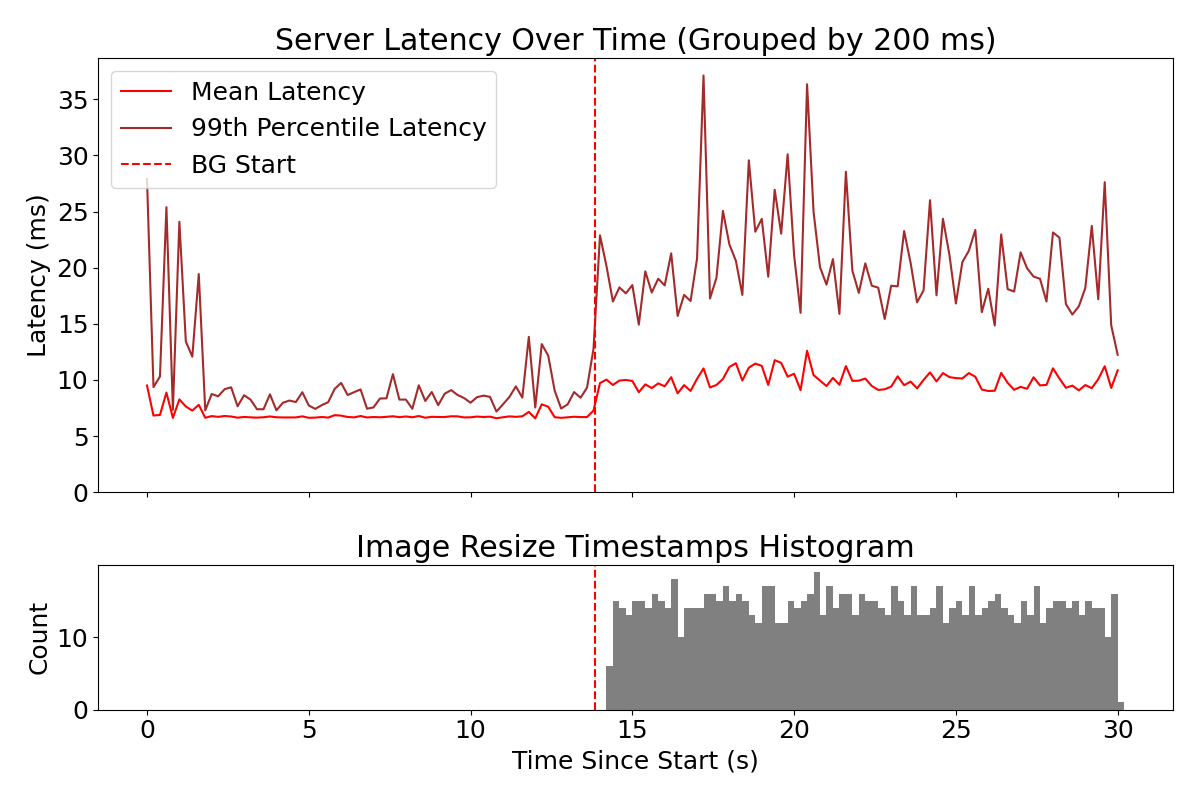
\includegraphics[width=\columnwidth]{graphs/kubernetes-idle.png}
    \caption{ \schedidle{} does better than \cgroups{}' weights, but not as well
    as the priority scheduling approach of \rtclass{} and \schedbe{}
    }\label{fig:kubernetes-idle}
\end{figure}

\autoref{fig:srv-bg-idle} shows the result of running the best effort job in the
microbenchmark in \schedidle{}, as well as a graph that compares the low load
setting of the standard \cgroups{} weight, \schedbe{}, and \schedidle{}. Average
latency still increases from $\sim$6ms to $\sim$8ms in the low load setting.
Although this increase is smaller than the original increase to $\sim$15ms using
the standard weight interface, it is still high compared to the 0ms increase
that \schedbe{} achieves. \autoref{fig:kubernetes-idle} shows similar results
for the Kubernetes experiment.

This is because \schedidle{} does not perform the \exit{} check. This means that
the following scenario can occur: all the cores are running server threads when
a new request comes in on core 2. It performs the \entry{} check, sees that all
cores are currently running high weight processes, and enqueues the new thread
itself. A millisecond or two later, the server thread on core 4 completes the
request and blocks on the next read. Core 4, having nothing else to run, starts
running the best effort job. An \exit{} check would have prevented this by
adding another check on core 4 before starting to run the BE process, which
would have found the queued thread on core 2.